\documentclass[a4]{article}
\usepackage[utf8]{inputenc}
\usepackage[french]{babel}
\usepackage{listings}
\usepackage{color}
\usepackage{graphicx}
\usepackage[T1]{fontenc}
\usepackage{pdfpages}
\usepackage{geometry}
\geometry{hmargin=2.5cm,vmargin=2.5cm}

\definecolor{mygreen}{rgb}{0,0.6,0}
\definecolor{mygray}{rgb}{0.5,0.5,0.5}
\definecolor{mymauve}{rgb}{0.58,0,0.82}

\lstset{
  backgroundcolor=\color{white},   % choose the background color; you must add \usepackage{color} or \usepackage{xcolor}
  basicstyle=\footnotesize,        % the size of the fonts that are used for the code
  breakatwhitespace=false,         % sets if automatic breaks should only happen at whitespace
  breaklines=true,                 % sets automatic line breaking
  captionpos=b,                    % sets the caption-position to bottom
  commentstyle=\color{mygreen},    % comment style
  deletekeywords={...},            % if you want to delete keywords from the given language
  escapeinside={\%*}{*)},          % if you want to add LaTeX within your code
  extendedchars=true,              % lets you use non-ASCII characters; for 8-bits encodings only, does not work with UTF-8
  frame=L,	                       % adds a frame around the code
  keepspaces=true,                 % keeps spaces in text, useful for keeping indentation of code (possibly needs columns=flexible)
  keywordstyle=\color{blue},       % keyword style
  language=C,                 	   % the language of the code
  otherkeywords={*,...},           % if you want to add more keywords to the set
  numbers=none,                    % where to put the line-numbers; possible values are (none, left, right)
  numbersep=5pt,                   % how far the line-numbers are from the code
  numberstyle=\tiny\color{mygray}, % the style that is used for the line-numbers
  rulecolor=\color{black},         % if not set, the frame-color may be changed on line-breaks within not-black text (e.g. comments (green here))
  showspaces=false,                % show spaces everywhere adding particular underscores; it overrides 'showstringspaces'
  showstringspaces=false,          % underline spaces within strings only
  showtabs=false,                  % show tabs within strings adding particular underscores
  stepnumber=2,                    % the step between two line-numbers. If it's 1, each line will be numbered
  stringstyle=\color{mymauve},     % string literal style
  tabsize=2,	                   % sets default tabsize to 2 spaces
  title=\lstname                   % show the filename of files included with \lstinputlisting; also try caption= instead of title
}
%gestion des caractères latins
\lstset{literate=
  {á}{{\'a}}1 {é}{{\'e}}1 {í}{{\'i}}1 {ó}{{\'o}}1 {ú}{{\'u}}1
  {Á}{{\'A}}1 {É}{{\'E}}1 {Í}{{\'I}}1 {Ó}{{\'O}}1 {Ú}{{\'U}}1
  {à}{{\`a}}1 {è}{{\`e}}1 {ì}{{\`i}}1 {ò}{{\`o}}1 {ù}{{\`u}}1
  {À}{{\`A}}1 {È}{{\'E}}1 {Ì}{{\`I}}1 {Ò}{{\`O}}1 {Ù}{{\`U}}1
  {ä}{{\"a}}1 {ë}{{\"e}}1 {ï}{{\"i}}1 {ö}{{\"o}}1 {ü}{{\"u}}1
  {Ä}{{\"A}}1 {Ë}{{\"E}}1 {Ï}{{\"I}}1 {Ö}{{\"O}}1 {Ü}{{\"U}}1
  {â}{{\^a}}1 {ê}{{\^e}}1 {î}{{\^i}}1 {ô}{{\^o}}1 {û}{{\^u}}1
  {Â}{{\^A}}1 {Ê}{{\^E}}1 {Î}{{\^I}}1 {Ô}{{\^O}}1 {Û}{{\^U}}1
  {œ}{{\oe}}1 {Œ}{{\OE}}1 {æ}{{\ae}}1 {Æ}{{\AE}}1 {ß}{{\ss}}1
  {ű}{{\H{u}}}1 {Ű}{{\H{U}}}1 {ő}{{\H{o}}}1 {Ő}{{\H{O}}}1
  {ç}{{\c c}}1 {Ç}{{\c C}}1 {ø}{{\o}}1 {å}{{\r a}}1 {Å}{{\r A}}1
  {€}{{\EUR}}1 {£}{{\pounds}}1
}
%definition d'un syle pour les documents texte
\lstdefinestyle{txt}{
	frame=none,
	numbers=none,
	stringstyle=\color{black},
}

\begin{document}
	\title{\Huge{\textbf{Cahier Des Specifications}}}
	\author{Alabi Steve - Benyamna Younes - Capdenat Nicolas- \\
		Chouipe Thibaut - El Harti Zakaria - Lienhardt Florian \\ \\ \\
		Chef de projet : Benyamna Younes \\ \\ \\ 
		Sous la direction de Mme Kloul \\ \\ \\ \\
		Outil automatique de décryptage \\ \\ \\}
		

	\begin{titlepage}
		\maketitle
		\vspace{20em}
		\begin{center}
\includegraphics{logo_uvsq.jpg}\end{center}
	\end{titlepage}
	\section{Introduction}
Dans le cadre de notre troisième année de licence nous devons réaliser une application d'aide au
décryptage par la méthode de Substitution ainsi que celle de Vigenère.
Nous vous avons donc proposé l'application Dcrypt qui permet de décrypter 
mais également crypter un texte ou même de faire une analyse fréquentielle sur un texte.
Pour cela, nous avons rédigé un cahier des charges afin de clarifier les objectifs et les 
exigences de ce projet. Dans la suite du cahier des charges, nous vous proposons donc
le cahier des spécifications.\\

Pour développer notre projet et après étude des besoins les arguments en faveur du langage C sont les suivants:\\

-Tout d'abord, le C permet d'utiliser des expressions et des opérateurs qui sont très proches du langage machine, 
il est donc possible de développer des programmes efficients et rapides.\\

-La portabilité est aussi un argument de choix: En effet, en respectant le standard ANSI-C, il est possible d'utiliser
le même programme sur tout autre système (autre hardware, autre système d'exploitation), simplement en le recompilant.\\

-De plus, pour assurer la maintenance du produit apres sa realisation et ce meme par des developpeurs qui ne sont
pas ceux d'origine, il faut un langage des plus utilisés et maitrisés\\

-Enfin, selon l'IEEE(*), le langage C est depuis 2016 le meilleur langage de 
programmation( de par sa forte croissance et sa demande par les employeurs). C'est aussi le langage n=1 pour le développement
d’applications d’entreprise, de bureau et d'applications scientifiques.\\

Nous avons également choisi une bibliothèque graphique du langage C: GTK+. Cette dernière nous permet de gérer efficacement
la navigation entre les differentes fenêtres
ainsi que nos accès memoires pour la sauvegarde et le chargement de nos fichiers. 
IEEE(*):  Institut des ingénieurs électriciens et électroniciens.
C'est la plus grande organisation professionnelle technique du monde de l'évolution de la technologie
	\section{Organigramme}
			\underline{Interface graphique :}     \hspace{5cm}  \underline{Cryptage Substitution :}\\
			- bouton cryptage            \hspace{5.5cm}       -créer une clé aleatoirement\\
			- bouton decryptage         \hspace{5cm}        -crypter le message\\
			- bouton substitution\\
			- bouton Vigenère           \hspace{5.2cm}       \underline{Cryptage Vigenère :}\\
			- affichage de texte(complet et partiel)  \hspace{2.2cm} -crypter le message\\
			- affichage pour la clé de substitution\\
			- bouton Francais(decryptage)   \hspace{3.5cm}     \underline{Decryptage Substitution :}\\
			- bouton Anglais(decryptage)    \hspace{3.5cm}     -decrypter le message\\
			- affichage pour l'analyse fréquentielle\\
			- charger un fichier texte       \hspace{4.2cm}  \underline{Analyse fréquentielle :}\\
			- sauvegarder un fichier texte     \hspace{3.8cm}  -analyse frequentielle sur texte donné\\
			- créer un nouveau fichier texte(resultats)\\
			- Demander clef de Vigenère\\
			
			\underline{Decryptage Vigenère :}\\
			-decrypter le message
			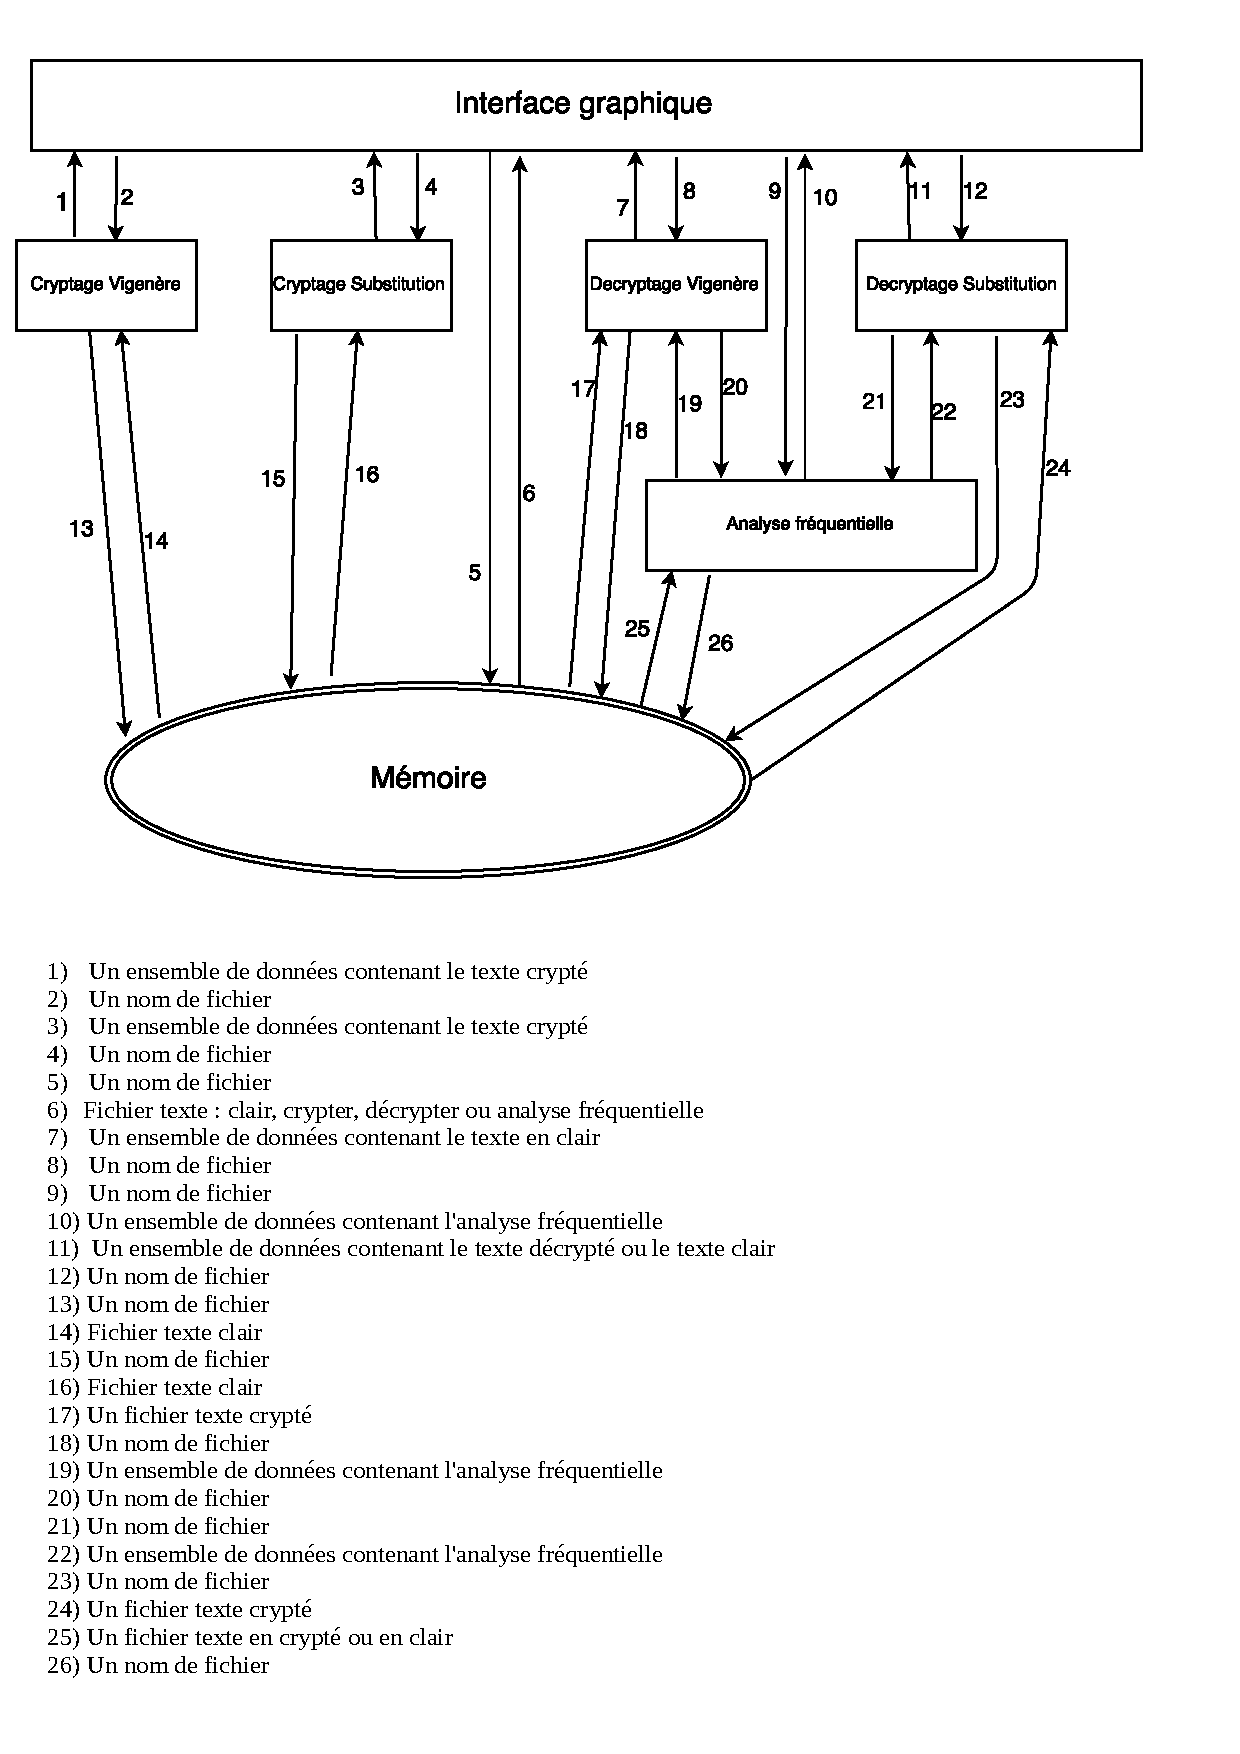
\includepdf[scale=0.7]{organigramme_final.pdf}
			
			
	\section{Signatures et Explications des methodes}
		\subsection{Diagramme des fonctions des differents modules}
		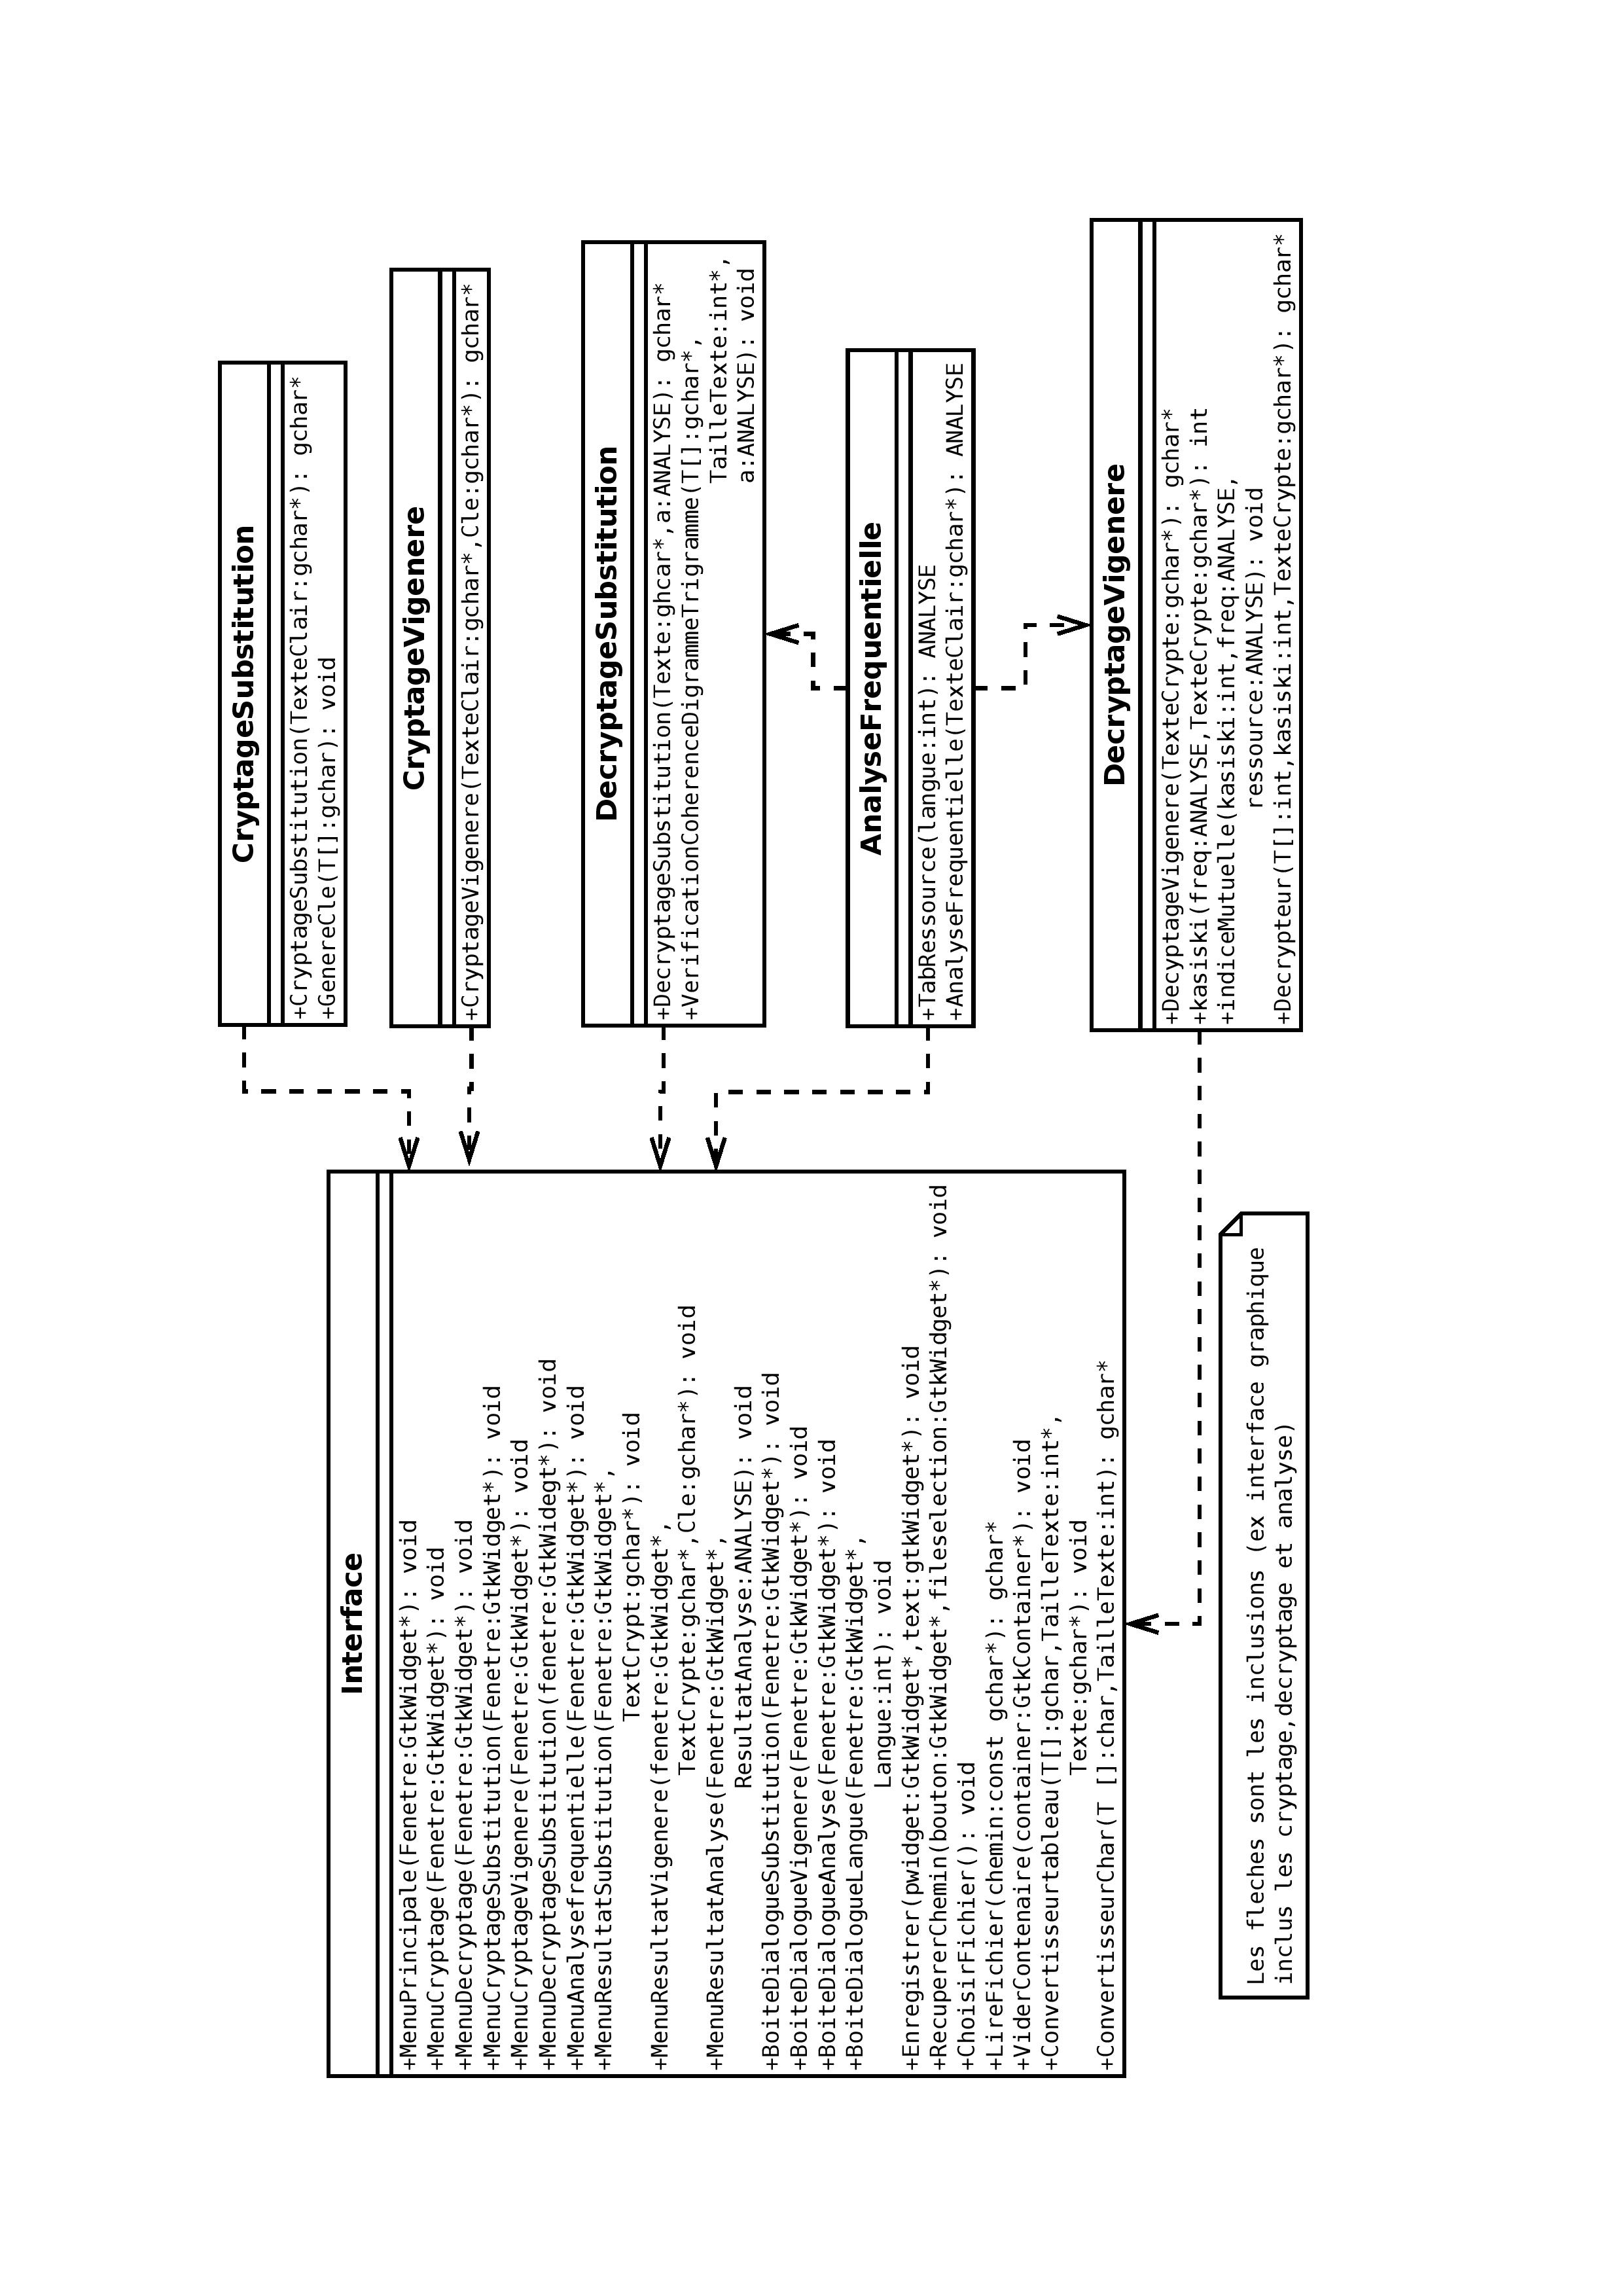
\includegraphics[scale=0.8]{diaa.jpg}
		\subsection{Structures et nouveaux types}
		Le gchar* est une chaîne de caractères, on utilise pas char* car dans la bibliothèque
		GTK+ l'affichage d'un texte se fait avec gchar*.\\
		
		les widgets (GTKWidget) sont les boutons, les zones de texte, les menus, enfin.. à peu 
		près tout ce qui constitue une interface.\\
		
		la seule  variable globale utilisée dans notre programme est Fenetre. Elle nous permet de
		conserver la fenêtre principale de notre application:\\
		GtkWidget *Fenetre; \\
		
	struct phoneme\{\\
		int frequence;\\
		gchar* nom;\\
	\}PHONEME;\\
	Cette structure représente les digrammes ou trigrammes et leurs fréquences.\\
	
	struct analyse\{ \\
		int nb //nbre de lettre \\
		float occ[25];\\
		PHONEME di[];\\
		PHONEME tr[];\\
		gchar* pgor;\\
	\}ANALYSE;\\
	Cette structure correspond aux caractéristiques d'un texte. Elle sera remplie lors de
	l'appel de la fonction "AnalyseFrequentielle". Ainsi, on connaitra
	le nombre de caractères dans celui-ci, les digrammes/trigrammes, la plus grande occurence
	rencontrée et la frequence d'apparition de chaque lettre.\\
	
	struct ressourceslangue\{ \\
		float occ[25];\\
		PHONEME di[];\\
		PHONEME tr[];\\
	\}RESSOURCESLANGUE;\\
	Cette structure correspond aux caractéristiques d'une langue. On connaitra
	les digrammes/trigrammes et la fréquence d'apparition de chaque lettre dans la langue choisie.
		\subsection{Signatures}
		
	
	\subsubsection{Analyse Frequentielle}
	ANALYSE TabRessource(int langue);\\
		La fonction prend en entrée un entier correspondant à la langue(francais ou anglais)
		et va ainsi remplir la structure "ANALYSE" et ses attributs suivants:
		la fréquence d'apparition de chaque lettre dans la langue choisie ainsi que les digrammes
		et les trigrammes.\\
		
		
		
	ANALYSE AnalyseFrequentielle(gchar* TexteClair)\\
		la fonction prend en entrée le texte clair a analyser et va ainsi remplir la structure "ANALYSE" et 
		ses attributs suivants:
		le nombre de lettres, la fréquence d'apparition de chaque lettre, les digrammes, les trigrammes
		et la plus grande occurence rencontrée.\\
		
	\subsubsection{Cryptage Substitution}
	gchar* CryptageSubstitution(gchar* TexteClair);\\
		Cette fonction permet de crypter un texte avec la méthode de Substitution\\
		Pour cela, elle prend en entrée une chaine de caractères qui correspond au texte clair.\\
		En sortie, le texte crypté sera sous forme de chaine de caractères.\\
		Le texte a crypter se trouve dans un tableau que nous allons parcourir. Et pour chaque caractere 
		nous allons aller lire dans un autre tableau [2][26] ou la premiere ligne correspond a l'alphabet
		de base et la deuxième celui de substitution(le nouveau). Ainsi, nous regardons la lettre dans 
		le premier tableau (du texte a crypter), on bascule dans le deuxieme tableau et trouve ce caractere dans la
		première ligne, puis on regarde sa lettre de substitution, et enfin on remplace dans le premier tableau 
		la lettre de base par ce caractère de substitution.
		
	void GenereCle(gchar T[]);\\
		génère une clé(alphabet) aléatoirement.
	
	\subsubsection{Decryptage Substitution}
	gchar* DecryptageSubstitution( gchar* texte, ANALYSE a)\\
		Prend en argument un texte crypté.\\
		Aprés avoir appelé la fonction d'analyse fréquentielle, cette fonction va, 
		dans une boucle, comparer les résultats de l'analyse frequentielle à l'alphabet
		 correspondant à la langue choisie et remplacer une lettre du message crypté 
		 par la lettre qu'elle semble crypter grace à une conjecture basée sur les 
		 fréquences des lettres les plus utilsés et complétée par l'analyse des digrammes 
		 et trigrammes. Cette fonction appelera ensuite la fonction VerificationCoherenceDigrammeTrigramme.\\
		Retourne en sortie le texte décrypté (gchar*).\\


	void VerificationCoherenceDigrammeTrigramme(gchar* T[], int *TailleTexte, ANALYSE a)\\
		Prend en argument le texte crypté en cours de décryptage.\\
		Cette fonction va parcourir le texte en cours de décryptage pour vérifier que les lettres trouvées 
		ne forment pas de digramme ou trigramme inabituels. Si c'est le cas elle proposera à l'utilisateur 
		de corriger le décryptage du texte ou le corrigera d'elle-même.\\
		Retourne en sortie le texte crypté en cours de décryptage( gchar*).\\
	
	
	\subsubsection{Decryptage Vignere}
	gchar* DecryptageVigenere(gchar* TexteCrypte);\\
		Cette fonction prend un texte crypté par le chiffrement de Vigenère \\
		et renvoie un texte clair et lisible par l'utilisateur.\\
	
	int Kasiski(ANALYSE freq, gchar* TexteCrypte);\\
		Cette fonction cherche les différentes distances de PGOR(Plus Grande Occurence Rencontrée) et effectue
		le PGCD de ces distances. Elle renvoie ce résultat sous forme d'un entier (qui représente la taille du mot clé cherché).\\
	
	void indiceMutuelle(int kasiski, ANALYSE freq, ANALYSE ressource);\\
		Cette fonction calcule les indices de coïncidences mutuelles et les stocke sous forme d'un tableau tab[25][kasiski].\\
		Elle parcourt et compare les 26 valeurs de chaque ligne afin de reperer celles qui sont proches de 0,065 (une par ligne).\\
		Elle renvoie l'indice de chacunes des valeurs valides dans un tableau a une dimension. \\
	
	gchar* decrypteur( int T[], int kasiski, gchar* TexteCrypte);\\
		Cette fonction soustrait la valeur du mot clef (tableau renvoyé par indiceMutuelle) au texte crypté.\\
		Elle va repeter la suite de nombre composant le mot clef jusqu'a la fin du texte afin de toujours pouvoir
		soustraire une valeur du mot clé a une valeur du texte crypté.\\
		Elle renvoie le texte claire.\\
		
		\subsubsection{Cryptage Vignere}
	gchar* CryptageVigenere(gchar* TexteClair, gchar* Cle);\\
		Cette fonction permet de crypter un texte avec la methode de Vigenere\\
		Elle prend en argument le texte clair et la clé qui sont tout les deux des chaines de caractères.\\
		La fonction renverra le texte crypté\\
		On construit un tableau [3][taille texte]. En première ligne on trouvera le texte a crypter, 
		en 2e la clé (qu'on repetera de facon a couvrir toute la 1e ligne(message a chiffrer)) et enfin 
		en 3e ligne le resultat de l'addition des caracteres des deux premieres lignes le tout modulo 
		26(c'est a dire le texte maintenant crypté).
		
		\subsubsection{Interface Graphique}
		Dans ce module nous allons utiliser plusieurs menus pour afficher notre application et naviguer 
		entre les menus pour cela nous allons créer plusieurs procédures qui vont afficher les menus  
		
		Les Menus\\
		
	void MenuPrincipal(GtkWidget *Fenetre);\\
		Cette procédure permet d'afficher le menu principal.\\
		Elle prend en argument la fenetre qui sera le contenaire(des boutons et labels).\\
		Cette procédure ne renvoie rien .\\
	
	void MenuCryptage(GtkWidget *Fenetre);\\
		Cette procédure permet d'afficher le menu de cryptage.\\
		Elle prend en argument la fenetre qui sera le contenaire(des boutons et labels).\\
		Cette procédure ne renvoie rien .\\
	
	void MenuDecryptage(GtkWidget *Fenetre);\\
		Cette procédure permet d'afficher le menu de decryptage.\\
		Elle prend en argument la fenetre qui sera le contenaire(des boutons et labels).\\
		Cette procédure ne renvoie rien .\\
	
	void MenuCryptageSubstitution(GtkWidget *Fenetre);\\
		Cette procédure permet d'afficher le menu de cryptage par la méthode de substitution.\\
		Elle prend en argument la fenetre qui sera le contenaire(des boutons et labels).\\
		Cette procédure ne renvoie rien .\\
	
	void MenuCryptageVigenere(GtkWidget *Fenetre);\\
		Cette procédure permet d'afficher le menu de cryptage par la méthode de vigenere.\\
		Elle prend en argument la fenetre qui sera le contenaire(des boutons et labels).\\
		Cette procédure ne renvoie rien .\\
	
	void MenuDecryptageSubstitution(GtkWidget *Fenetre);\\
		Cette procédure permet d'afficher le menu de decryptage par la méthode de substitution.\\
		Elle prend en argument la fenetre qui sera le contenaire(des boutons et labels).\\
		Cette procédure ne renvoie rien .\\
	
	void MenuDecryptageVigenere(GtkWidget *Fenetre);\\
		Cette procédure permet d'afficher le menu de decryptage par la méthode de vigenere.\\
		Elle prend en argument la fenetre qui sera le contenaire(des boutons et labels).\\
		Cette procédure ne renvoie rien .\\
	
	void MenuAnalyseFrequentielle(GtkWidget *Fenetre);\\
		Cette procédure permet d'afficher le menu d'analyse frequentielle.\\
		Elle prend en argument la fenetre qui sera le contenaire(des boutons et labels).\\
		Cette procédure ne renvoie rien .\\
	
	void MenuResultatSubstitution(GtkWidget *Fenetre, gchar* Textcrypt);\\
		Cette procédure permet d'afficher le menu du resultat du decryptage par la methode de substitution.\\
		Elle prend en argument la fenetre qui sera le contenaire(des boutons et labels).\\
		Cette procédure ne renvoie rien .\\
	
	void MenuResultatVigenere(GtkWidget *Fenetre, gchar* Textcrypt, gchar* cle);\\
		Cette procédure permet d'afficher le menu du resultat du decryptage par la methode de vigenere.\\
		Elle prend en argument la fenetre qui sera le contenaire(des boutons et labels).\\
		Cette procédure ne renvoie rien .\\
	
	void MenuResultatAnalyse(GtkWidget *Fenetre);//rajouer le texte\\
		Cette procédure permet d'afficher le menu du resultat de l'analyse frequentielle.\\
		Elle prend en argument la fenetre qui sera le contenaire(des boutons et labels).\\
		Cette procédure ne renvoie rien .\\
	
	void BoiteDialogueSubstitution(GtkWidget *Fenetre);\\
		Cette procédure affiche une zone de texte qui nous permet de rentrer le texte à crypter par substitution.\\
		Elle prend en argument la fenêtre.\\
	
	void BoiteDialogueVigenere(GtkWidget *Fenetre);\\
		Cette procédure affiche deux zones de texte qui permettent de rentrer le texte à crypter et la cle qui permet d'effectuer le chiffrement.\\
		Elle prend en argument une fenêtre.\\
		
	void BoiteDialogueAnalyse(GtkWidget *Fenetre);\\
		Cette procédure affiche une zone de texte qui permet de rentrer le texte sur lequel effectuer une analyse fréquentielle.\\
		Elle prend en argument une fenêtre.\\
		
	void BoiteDialogueLangue(GtkWidget *Fenetre,int langue);\\
		Cette procédure nous permet de choisir la langue (0:francais , 1:anglais).\\
		Elle prend en argument une fenêtre.\\
		
	nous aurons peut-être besoin d'autres menus au cours de notre application(pour un meilleur affichage ou ameliorations) 
	//menu pour la langue
	
	Les Enregistrement/Chargements\\
	
	void Enregistrer (GtkWidget *pwidget, GtkWidget *text );\\
		Cette procédure permet de sauvegarder le texte obtenue.\\
		Elle prend en argument une fenetre et le texte à sauvegarder.\\
		Cette procédure ne renvoie rien.\\
	
	void RecupererChemin(GtkWidget *bouton, GtkWidget *fileselection);\\
		Cette procédure permet de recuperer le chemin d'accés d'un fichier.\\
		Elle prend en argument une fenetre et une deuxieme fenetre (pour les fenetres de selections de fichier)\\
		Cette procédure appel\\

	void ChoisirFichier();\\
		Cette procédure nous permet de selectionner un fichier à charger (fichier qui contient le texte clair ou 		crypter)\\

		
	gchar* LireFichier(const gchar* chemin);\\
		Cette fonction permet de recuperer le texte qui est dans un fichier, pour cela nous donnons en argument un chemin de fichier.\\
	
	Autres\\
	
	void ViderContenaire(GtkContainer * container);\\
		Cette procédure nous permet de vider le contenu de la fenetre, cele nous permet de travailler avec une seule fenêtre.\\
		Cette procédure prend en argument la fenêtre à vider.\\
	void ConvertisseurTableau(gchar T[],int *TailleTexte,gchar* Texte);\\
		enlever accent et espace, et mettre dans un tableau\\
	 
	gchar* ConvertisseurChar(char T[],int TailleTexte); \\
		Parcours d'un tableau donné et le retourne en chaine de caracteres\\
		
	
	\section{Conclusion}
	
	Pour conclure, la rédaction de ce cahier des spécifications est une étape importante pour la réalisation du projet
	et plus précisément permet d'indiquer comment réaliser le besoin.\\
	
	Elle se situe après l'étape de conception (cahier des charges) et avant l'étape de réalisation (codage).\\
	
	Ce cahier permet donc de répondre de manière spécifique aux différentes reponses apportées, notamment les données en entrée
	ou en sortie des fonctions/procédures qui composent nos modules.\\
	
	Le diagramme résume les fonctions/procédures présentes dans chaque module ainsi que les liens d'inclusion.\\
	
	Maintenant que tout ces paramètres ont été définis et que l'équipe est d'accord sur l'architecture de l'application, nous allons
	passer à l'implémentation en respectant tout les règles fixées par le cahier des charges et des spécifications.
	
	
\end{document}
